% the following command is only required if the thesis is written in german
\RequirePackage[ngerman=ngerman-x-latest]{hyphsubst}

\documentclass[
  ngerman, % change to ngerman for german theses
  symmetric, % use two-side for booklike layouts
  numbers=noenddot % remove trailing dots in chapter/section/... enumeration
]{tudscrreprt}

\usepackage[T1]{fontenc}
\usepackage[utf8]{inputenc}
\usepackage[
  ngerman % change to ngerman for german theses
]{babel}
\usepackage{isodate}
\usepackage{pdfpages}
\usepackage{listings}
\usepackage[toc, page]{appendix}
\usepackage{hyphenat}

\usepackage[
  style=alphabetic,
  backend=biber,
  url=false,
  doi=false,
  isbn=false,
  hyperref,
]{biblatex}
% configure the location of the biblatex file
\addbibresource{bibliography.bib}
\AtEveryBibitem{%
  \clearfield{note}%
}

% make all links clickable but hide ugly boxes
\usepackage[hidelinks]{hyperref}
% automatically insert Fig. X in the text with \cref{..}
\usepackage[capitalise,nameinlink,noabbrev]{cleveref}

\usepackage[colorinlistoftodos,prependcaption,textsize=tiny]{todonotes}

\usepackage{graphicx}
\graphicspath{ {./images/} }

\usepackage{svg}

% if you need mathy stuff
\newtheorem{lem}{Lemma}
\crefname{lem}{Lemma}{Lemmas}
\newtheorem{thm}{Theorem}
\crefname{thm}{Theorem}{Theorems}
\newtheorem{defs}{Definition}
\crefname{defs}{Def.}{Defs.}

\usepackage{blindtext}

%\usepackage{tudscrsupervisor} % if you want to copy the sources of the task description into the thesis

\usepackage{csquotes}

\usepackage{caption}
\captionsetup{font=normalfont,labelfont=normalfont,labelsep=space}
\usepackage{floatrow}
\floatsetup{font=normalfont}
\floatsetup[table]{style=plaintop}
\captionsetup{singlelinecheck=off,format=hang,justification=raggedright}
\DeclareCaptionSubType[alph]{figure}
\DeclareCaptionSubType[alph]{table}
\captionsetup[subfloat]{labelformat=brace,list=off}

\usepackage{booktabs}
\usepackage{array}
\usepackage{tabularx}
\usepackage{tabulary}
\usepackage{tabu}
\usepackage{longtable}
\usepackage{multirow}

\usepackage{quoting}

\usepackage[babel]{microtype}

\usepackage{xfrac}

\usepackage{enumitem}
\setlist[itemize]{noitemsep}

\usepackage{ellipsis}
\let\ellipsispunctuation\relax

\usepackage{listings}
\usepackage{xcolor}

\definecolor{commentsColor}{rgb}{0.497495, 0.497587, 0.497464}
\definecolor{keywordsColor}{rgb}{0.000000, 0.000000, 0.635294}
\definecolor{stringColor}{rgb}{0.558215, 0.000000, 0.135316}

\lstset{ %
  backgroundcolor=\color{white},   % choose the background color; you must add \usepackage{color} or \usepackage{xcolor}
  basicstyle=\footnotesize,        % the size of the fonts that are used for the code
  breakatwhitespace=false,         % sets if automatic breaks should only happen at whitespace
  breaklines=true,                 % sets automatic line breaking
  captionpos=b,                    % sets the caption-position to bottom
  commentstyle=\color{commentsColor}\textit,    % comment style
  deletekeywords={...},            % if you want to delete keywords from the given language
  escapeinside={\%*}{*)},          % if you want to add LaTeX within your code
  extendedchars=true,              % lets you use non-ASCII characters; for 8-bits encodings only, does not work with UTF-8
  frame=tb,	                   	   % adds a frame around the code
  keepspaces=true,                 % keeps spaces in text, useful for keeping indentation of code (possibly needs columns=flexible)
  keywordstyle=\color{keywordsColor}\bfseries,       % keyword style
  language=Python,                 % the language of the code (can be overrided per snippet)
  otherkeywords={*,...},           % if you want to add more keywords to the set
  numbers=left,                    % where to put the line-numbers; possible values are (none, left, right)
  numbersep=5pt,                   % how far the line-numbers are from the code
  numberstyle=\tiny\color{commentsColor}, % the style that is used for the line-numbers
  rulecolor=\color{black},         % if not set, the frame-color may be changed on line-breaks within not-black text (e.g. comments (green here))
  showspaces=false,                % show spaces everywhere adding particular underscores; it overrides 'showstringspaces'
  showstringspaces=false,          % underline spaces within strings only
  showtabs=false,                  % show tabs within strings adding particular underscores
  stepnumber=1,                    % the step between two line-numbers. If it's 1, each line will be numbered
  stringstyle=\color{stringColor}, % string literal style
  tabsize=2,	                   % sets default tabsize to 2 spaces
  title=\lstname,                  % show the filename of files included with \lstinputlisting; also try caption instead of title
  columns=fixed                    % Using fixed column width (for e.g. nice alignment)
}

\lstdefinelanguage{XML} % use with language = XML
{
  morestring=[b]",
  morestring=[s]{>}{<},
  morecomment=[s]{<?}{?>},
  morekeywords={xmlns,version,type}
}


 % code styles (listings)

% use this custom theorem for research questions
\newtheorem{researchquestion}{Forschungsfrage}
\crefname{researchquestion}{Forschungsfrage}{Forschungsfragen}

% use this custom environment for equations
\newenvironment{conditions}
  {\par\vspace{\abovedisplayskip}\noindent\begin{tabular}{>{$}l<{$} @{${}={}$} l}}
  {\end{tabular}\par\vspace{\belowdisplayskip}}

\usepackage{float}

% configure the name of your appendix
\renewcommand\appendixtocname{Anhang}
\renewcommand\appendixpagename{Anhang}

% use \tocless before a chapter/section/... in the
% appendix to hide it from the toc
\newcommand{\nocontentsline}[3]{}
\newcommand{\tocless}[2]{
  \bgroup\let\addcontentsline=\nocontentsline#1{#2}\egroup
}

\begin{document}

  % use uppercase roman letters for all pages until the introduction
  % this way, it is easier to identify how many pages the thesis has
  \pagenumbering{Roman}

  \faculty{Fakultät Informatik}
  \department{}
  \institute{Institut für Systemarchitektur}
  \chair{Professur für Rechnernetze}
  \title{%
    Dokumentation über den Neuaufbau der OUTPUT.DD App im WiSe 2020/21
  }

  \thesis{project} % the type of thesis you want to write

  \author{Philipp Matthes}
  \matriculationnumber{4605459}
  \matriculationyear{WiSe 2016/17}
  \dateofbirth{12.3.1997}
  \placeofbirth{Chemnitz}

  \course{Diplom Informatik (PO 2010)}

  \supervisor{%
    Dr. Thomas Springer
  }
  \maketitle

  \newpage

  % include the task definition if you want
  % \includepdf[pages=-]{task/task.pdf}
  % \newpage

  % for the order of the following sections please refer to
  % the recommendations for thesis structuring
  \confirmation

  \tableofcontents

  \listoffigures
  \addcontentsline{toc}{chapter}{\listfigurename}

  \listoftables
  \addcontentsline{toc}{chapter}{\listtablename}

  % this is where your thesis lives
  \chapter{Einleitung}\label{ch:einleitung}\pagenumbering{arabic}

OUTPUT.DD ist eine jährlich stattfindende Projektschau, auf welcher in der Fakultät Informatik der Technischen Universität Dresden wissenschaftliche Projekte von Studenten, Firmen und Mitarbeitern präsentiert und ausgestellt werden. Begleitend zur Projektschau wird den Besuchern der Veranstaltung jeweils eine App für iOS und Android zur Verfügung gestellt. Die Apps dienen dabei selbst nicht nur als Plattform, über welche Nutzer den zeitlichen und topografischen Veranstaltungsplan einsehen können, sondern auch als Integrationspunkt für verschiedene Forschungsprojekte aus den Bereichen Mediengestaltung, Application Development und Mobile Computing. So wird die Interaktion der Nutzer beispielsweise durch eine Gamification\footnote{Gamification. Einsatz von Spielelementen in einem Nicht-Spiel-Kontext.} motiviert und geleitet, oder die Bewegung des Nutzers auf der Messe über ein im Rahmen des Forschungsprojektes \enquote{Mapbiquitous} entstandenes Beaconing-Framework verfolgt, um das Besucheraufkommen zu analysieren und dem Nutzer eine interaktive Heatmap auf der Kartenansicht der Veranstaltung anzuzeigen. Außerdem nutzt die App das Offline-First-Prinzip aus dem Forschungsbereich Ubiquitäre Applikationen, bei dem die in der App angezeigten Daten koordiniert von einem Server-Backend synchronisiert werden, um bei einem Netzwerkausfall weiterhin so viele Funktionalitäten wie möglich zu unterstützen und die offline geschriebenen Daten bei der Wiederherstellung der Verbindung im Hintergrund zu aktualisieren. Im Sommer 2020 wurden für die beiden Apps jeweils Datenbank-Frameworks für die NoSQL-Datenbank Couchbase entwickelt, welche architekturell im Repository-Pattern\footnote{Repository-Pattern. Architekturelles Pattern zur Abstraktion und Separation von Datenbankabfragen durch die Bereitstellung von CRUD-Operationen (Create, Read, Update, Delete).} umgesetzt wurden und zur Synchronisation der Daten so genannte Replikatoren bereitstellen, die über einen Synchronisationsdienst mit dem Couchbase Backend-Server kommunizieren.

\section{Problemstellung}

Da die OUTPUT.DD Apps in den vergangenen Jahren noch auf ein anderes, auf Realm basierendes, Datenbank-Backend aufsetzten, musste eine Substitution des Datenbank-Backends analysiert, geplant, durchgeführt und getestet werden.

Durch die sukzessive funktionelle Erweiterung der Apps über mehrere Jahre unter verschiedenen Teams mit jeweils unterschiedlichen Qualitätsansprüchen, Zeitvorgaben und Kenntnisständen bildeten sich außerdem mehrere Probleme in der Implementation heraus, die durch einen Audit der iOS-Codebasis am 5.4.2020 identifiziert werden konnten:

\begin{itemize}
  \item \textbf{Strukturelle Antipatterns}, darunter eine schwer nachvollziehbare Ordner- und Dateistrukturierung, das Nichtvorhandensein einer Separation in Module, sowie die Vermischung von abkapselbaren externen und internen Frameworks mit der primären Codebasis
  \item \textbf{Architekturelle Antipatterns}, wie beispielsweise die \enquote{Verschmutzung}\footnote{Verschmutzung. Von Englisch \enquote{Pollution}, wird oft als Fachbegriff verwendet, um die Degradation der Codequalität durch fehlpositionierte Codefragmente zu verbildlichen.} des Codes durch globale Erweiterungen von Datenbankmodellen an unerwarteten Stellen
  \item \textbf{Weitere Probleme}, darunter die Ignorierung von Sicherheitsrisiken durch das Ausschalten von Dependency-Warnings, an einer Stelle auch die Fehlverwendung von View-Life-Cycles, das allgemeine Vorhandensein Code Smells und die technische Alterung des Objective-C Codes.
\end{itemize}

\section{Ziele der Projektarbeit}

Da OUTPUT.DD 2020 vor dem Hintergrund der Sars-CoV-2 Pandemie nicht stattfand, wurde im Projektteam beschlossen, diese Probleme durch eine Neuimplementation der Applikation zu beheben, mit dem beiläufigen Ziel, auch das neue Datenbank-Backend zu integrieren. Im Projektteam wurde entschieden, die Apps mit den jeweils aktuellsten Technologien neu zu implementieren, darunter eine Reimplementation der Android-App mit der Programmiersprache Kotlin, sowie eine (in dieser Arbeit näher beschriebenen) Reimplementation der iOS-App mit der Programmiersprache Swift und dem 2019 von Apple eingeführten UI-Framework SwiftUI, welches eine deklarative Ansichtserstellung ermöglicht. Hierdurch sollten die Apps technisch und visuell modernisiert werden. Bei der Reimplementation sollten die oben beschriebenen Probleme durch die Einführung klarer Architektur- und Strukturpatterns möglichst vermieden werden, sowie außerdem konkrete Strategien und Richtlinien entworfen werden, um ein Wiedereintreten dieser Probleme zu vermeiden und somit zukünftigen Projektteams die Weiterentwicklung der Apps zu erleichtern. Diese Arbeit soll einen chronologischen Überblick darüber geben, welche Schritte gegangen wurden, um diese Ziele zu erreichen, und die Endprodukte schließlich evaluieren.

  \chapter{Grundlagen}\label{ch:grundlagen}

In diesem Kapitel sollen zunächst wichtige theoretische Grundlagen erklärt werden, die zum Verständnis der in den nachfolgenden Kapiteln beschriebenen Projektbearbeitungsschritte und -entscheidungen notwendig sind.

\section{Swift und SwiftUI}

Eine Festlegung, die bereits vor der Reimplementation der Apps getroffen wurde, ist die Wahl von Swift als Hauptprogrammiersprache der zu erstellenden iOS App. Die Programmiersprache wurde 2014 von Apple veröffentlicht und ersetzt seitdem Objective-C als die von Apple empfohlene Objektorientierte Sprache zur Erstellung von Applikationen für das Apple-Ökosystem mit den Betriebssystemderivaten Mac OS, iOS und bspw. auch Watch OS (Apple Watch). In der aktuellen Version 5 setzt Swift vielseitig etablierte Konzepte aus modernen Programmiersprachen um und ist hierbei nach dem subjektiven Empfinden des Projektteams leicht verständlich, schnell zu erlernen, sowie sehr kompakt. Zusammen mit Swift 5 wurde SwiftUI als deklaratives UI-Framework 2019 veröffentlicht, ergänzend zum herkömmlichen Constraint-basierten Layouting über UIView(Controller) und XIB/Storyboard-Dateien. SwiftUI orientiert sich an Frameworks wie React, bei denen Ansichten im Code definiert werden können, wodurch die Erstellung und Modifikation von Ansichten direkt im Editor geschehen kann, ohne die Notwendigkeit von etwaiger Controller-Logik, die UI-Elemente mit Code-Elementen (z.B. über die Annotation \texttt{@IBAction}) verbindet. Dies vereinfacht den Implementationsprozess, bringt jedoch auch verschiedene neue Architektur- und Datenflusskonzepte mit sich, die zunächst verstanden werden müssen, um SwiftUI effektiv und zielorientiert nutzen zu können.

\section{Datenfluss- und Architekturpatterns in SwiftUI}

In der nachfolgenden Sektion sollen zunächst die wesentlichsten Grundlagen des Datenflusses in SwiftUI-Ansichten erläutert werden. Anschließend werden verschiedene Patterns vorgestellt, die sich im Implementationskonzept wiederspiegeln und auch zukünftig idealerweise weiter genutzt werden sollten.

\subsection{Darstellung von View-Daten}

Im Unterschied zum imparativen UI-Programmierkonzept, bei dem konkrete Elemente der Ansicht, wie bspw. Labels oder Textfelder imparativ konfiguriert und mit den darzustellenden Daten ausgestattet werden, referenziert eine SwiftUI Ansicht (\enquote{View}) die darzustellenden Daten direkt aus dem Code, da sie selbst deklarativ in Form von Code geschrieben werden kann.

\begin{figure}[H]
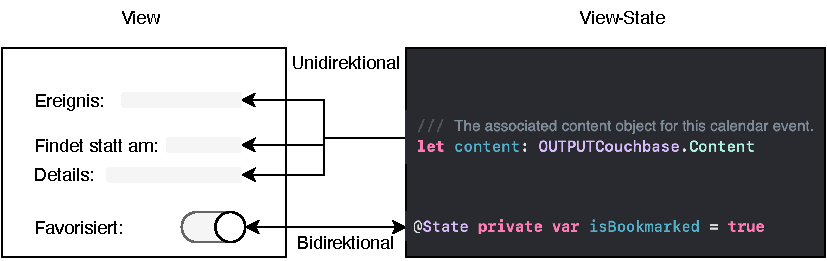
\includegraphics[width=\linewidth, bb=0 0 396 125]{swiftui.pdf}
\caption{Zwei wesentliche Arten des Datenflusses zwischen View und den in der View dargestellten Daten: unidirektional vs. bidirektional.}\label{fig:swiftui}
\end{figure}

\noindent \Cref{fig:swiftui} zeigt die zwei wesentlichsten Varianten, mithilfe derer Daten in der Ansicht dargestellt werden können: \textbf{unidirektional} und \textbf{bidirektional}. Bei der unidirektionalen Darstellung der Daten werden bei der Initialisierung der View die Daten im Konstruktor der View mitgegeben - da SwiftUI Views so genannte Structs sind, können die Daten im Verlauf der Zeit nicht mehr ändern (Struct-Felder sind \enquote{immutable}). SwiftUI rendert die assoziierten Elemente der View einmalig und verwendet diese nachfolgend zur Darstellung. Für viele Anwendungsfälle, in \Cref{fig:swiftui} anhang eines \enquote{Favorisieren-Buttons} illustriert, ist es jedoch notwendig, dass durch die View die dahinter liegenden Daten modifiziert werden. Hierfür wird der Property Wrapper \texttt{@State} bereitgestellt. Attribute, die hiermit ausgestattet werden, können während der Präsentation der View verändert werden. Eine Besonderheit hierbei ist, dass SwiftUI genau observiert, welche UI-Elemente durch das annotierte Attribut modifiziert oder konfiguriert werden, um bei einer Änderung des Attributs die entsprechenden Elemente neu zu rendern. Wird ein Datenattribut an eine Unteransicht weitergegeben, welche bspw. eine Detailansicht zu einem Objekt darstellt, dann wird das Attribut in der Unteransicht als \texttt{@Binding} referenziert.

\subsection{Coordinator-Pattern}

Um die Geschäftslogik der Anwendung von der Darstellungslogik weitestgehend zu separieren, kann das Coordinator-Pattern genutzt werden. Hierbei instanziiert die View ein eigenes Objekt, welches sie durch die \texttt{@StateObject} Annotation besitzt und kontrollieren kann, bspw. durch die Interaktion des Nutzers oder beim Erscheinen der Ansicht. Das Coordinator-Objekt macht die darzustellenden Datenattribute über die \texttt{@Published} Annotation nach außen verfügbar - so dass die View diese Datenattribute (ähnlich zu \texttt{@State} Datenattributen) verwenden und auf deren Änderungen reagieren kann.

\begin{figure}[H]
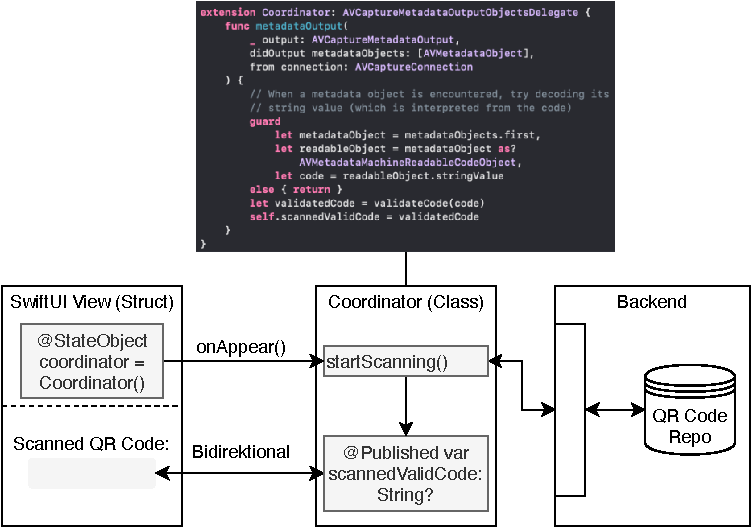
\includegraphics[width=\linewidth, bb=0 0 360 253]{coordinator.pdf}
\caption{Das Coordinator Pattern illustriert am Beispiel eines hypothetischen QR Code Scanners: Der Coordinator realisiert die Initialisierung des Scanners und die Validierung des Codes. Die View stellt den Code lediglich dar, sobald er gescannt wurde.}\label{fig:coordinator}
\end{figure}

\noindent In \Cref{fig:coordinator} ist das Pattern am Beispiel illustriert. Auch zu sehen ist hierbei, dass der Coordinator eine Klasse ist. Dies ist nützlich wenn bestimmte Protokolle (Swift-Interfaces) implementiert werden müssen, in diesem Beispiel \texttt{AVCaptureMetadataOutputObjectsDelegate} zur Reaktion auf gescannte QR Codes. In diesem Beispiel kann die View dieses Protokoll nicht implementieren, da das Protokoll implizit die Implementation durch eine Klasse erfordert.

\subsection{Environment-Pattern}

Als weiteres wichtiges Datenfluss-Pattern dient das Environment-Pattern. Hierbei wird, ähnlich zum Coordinator-Pattern, ein koordinierendes Umgebungsobjekt instanziiert und in der Besitz ergreifenden View als \texttt{@StateObject} markiert. Anschließend wird das Umgebungsobjekt im Environment der Unteransichten mitgegeben, über den ViewModifier \texttt{view.environmentObject()}. Dies ist zum Beispiel sinnvoll, wenn eine Unteransicht bestimmte Daten aus dem Kontext beziehen und/oder modifizieren möchte.

\begin{figure}[H]
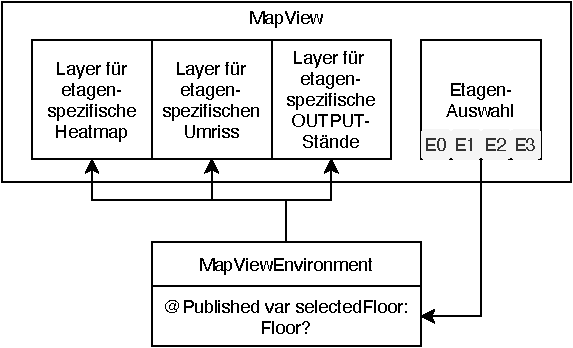
\includegraphics[width=0.75\linewidth, bb=0 0 275 167]{environment.pdf}
\caption{Das Environment Pattern illustriert am Beispiel der Map View: Die Map View erstellt ihr eigenes Environment und gibt dieses an ihre Unteransichten weiter. Somit kann die gewählte Etage von einer Unteransicht modifiziert werden, von anderen Unteransichten wird sie lediglich dargestellt.}\label{fig:environment}
\end{figure}

\noindent In \Cref{fig:environment} ist dieses Pattern am Beispiel illustriert. Ein großer Vorteil des Patterns ist, dass das über den ViewModifier weitergegebene Umgebungsobjekt transitiv an alle weiteren Unteransichten weitergeleitet wird, die sich möglicherweise in dieser Unteransicht befinden. Der Bezug des Objektes findet anschließend über \texttt{@EnvironmentObject var object} statt. Ein Problem hierbei ist, dass das Objekt nicht optional weitergegeben werden kann, was die Preview der SwiftUI Unteransichten erschwert. Die hierfür applizierte Lösung hierfür wird später im Konzeptkapitel näher beschrieben.

\subsection{View-Proxy-Pattern}

Die Grundlagen des Environment-Pattern und des Coordinator-Pattern können weiterhin genutzt werden, um bestimmte Bestandteile der Geschäftslogik im View-Proxy-Pattern zu separieren. Hierbei wird eine dedizierte View erstellt, deren Aufgabe es ist, bestimmte Datenverarbeitungsoperationen durchzuführen und bei Beendigung dessen die Produkte dieser Operation als Umgebungsobjekt bzw. Proxy-Objekt der inneren View bereitzustellen. Hierfür wird die innere View der Proxy View als \texttt{@ViewBuilder}-Closure übergeben. Ein klassisches Beispiel für das View-Proxy-Pattern ist der von SwiftUI standardmäßig bereitgestellte \texttt{GeometryReader}, welcher als View genutzt werden kann, um ein Proxy-Objekt für die Geometrie der View zu erstellen, bspw. um die Größe einer Ansicht zu bestimmen. Im Konzept der App wird dies später für die Initialisierung der Datenbank und Replikatoren adaptiert und an dieser Stelle noch einmal genauer beschrieben.

\subsection{Eventbasierte Datenflüsse}

Eventbasierte Datenflüsse stellen ein weiteres wichtiges Pattern für die Weitergabe von Daten dar. Bei den bisherigen Pattern wurden lediglich Methoden vorgestellt, mithilfe derer sich ein Datenfluss zwischen mehreren Views in \textit{derselben} View-Hierarchie realisieren lässt. In manchen Fällen ist es jedoch notwendig, dass bestimmte Datenverarbeitungsprozesse von der View-Hierarchie entkoppelt werden, beispielsweise bei periodischen Hintergrundprozessen. Um in diesem Fall dennoch bspw. eine entsprechende Meldung im UI anzuzeigen, können globale Events ausgelöst werden, die von Observern innerhalb der View aufgegriffen und zur Anzeige verarbeitet werden können. Hierbei kann das \texttt{NotificationCenter} genutzt werden, um Nachrichten auf einen Event-Bus zu pushen und innerhalb der View über einen so genannten \texttt{Publisher} zu empfangen. Auch dieses Pattern wird später noch an einem konkreten Beispiel im Rahmen des Implementationskonzeptes zu den Spiel-Errungenschaften gezeigt.


  \newpage

  % use lowercased roman page numbers for the appendix and the bibliography
  \pagenumbering{roman}

  \printbibliography[heading=bibintoc]\label{sec:bibliography}%

  \begin{appendices}
    \tocless\chapter{Appendix A}\label{appendix:a}

  \end{appendices}

\end{document}
